\chapter{Présentation du code de dimensionnement}

\section{Introduction}

L'objectif du code est de dimensionner la taille du stockage sensible. Pour faire cela, il nous faut fixer une largeur et profondeur, la température de l'air que l'on souhaite en sortie, puis le programme calculera la hauteur de l'échangeur. 

Pour qu'il le réalise, nous avons discrétisé notre problème et rentré les équations de la chaleur. De ce fait, il calcule la température de l'air au cours du temps et analysera sa température final en sortie. Si elle est supérieure à celle souhaité, il rajoutera un certain nombre de tubes sur la hauteur et recommencera jusqu'à atteindre la consigne voulu.

Le concept général étant vus, nous allons maintenant le décrire en détaille. Nous verrons son organigramme, les hypothèses que nous avons dû faire, les équations que nous avons écrit, les variables d'entrées et de sorties.


\section{Hypothèse simplificatrice}

	Nous allons présenter dans cette partie les hypothèses faites pour coder notre modèle afin que les résultats obtenue soit bon tout en gardant un code relativement simple.\\
	
	Premièrement, la turbulence a été négligé. La rencontre du fluide avec des tubes cylindriques parallèle à l'écoulement provoque en effet de forte turbulence. Cependant, cela permet de favoriser l'homogénéisation de la température dans l'air. Nous pouvons donc tourner cela à notre avantage puisque sa nous permet de représenter une seul maille d'air entre deux tube de Cofalite. En contre partie, elle augmente aussi les pertes de charge dans l'échangeur. \\
	
	
	Cependant, nous allons faire une deuxième hypothèse en négligeant ces pertes de charge qui conduise à un baisse de pression mais de manière assez négligeable.  \textcolor{red}{Faire un ptit truc EES pour vérifier que cela est vrai. il parait qu'il y a une petite formule dans le truc de bédécarrat ou l'on a trouvé la corrélation de H} 
	
	Pour finir, nous négligeons également les transferts par rayonnement. Même si nous avons des températures assez élevées, la complexité pour intégrer les équations de rayonnement dans ce code est très importante. Nous ne connaissons pas les facteurs de forme qu'il y a entre les tubes et nous devrions calculer l'absorptivité de l'air en fonction de la pression et température.

	Ces hypothèses nous ont menées au maillage décrit dans la section qui suit.




\newpage
\section{Le maillage}

Nous avons discrétisé en espace un élément de notre échangeur puis nous avons répété ce schéma sur la hauteur. Nous avons donc une hauteur d'échangeur qui est : hauteur = diamètre du Cofalite $\times$ nombre de tubes.

Nous avons discrétisé en volume constant le tube le Cofalite (voir le schéma \ref{maillage}) \\


Nous présentons ci-dessous les schémas avec les grandeurs caractéristiques :




\begin{figure}[!h]
\centering
\caption{Configuration Géométrique}
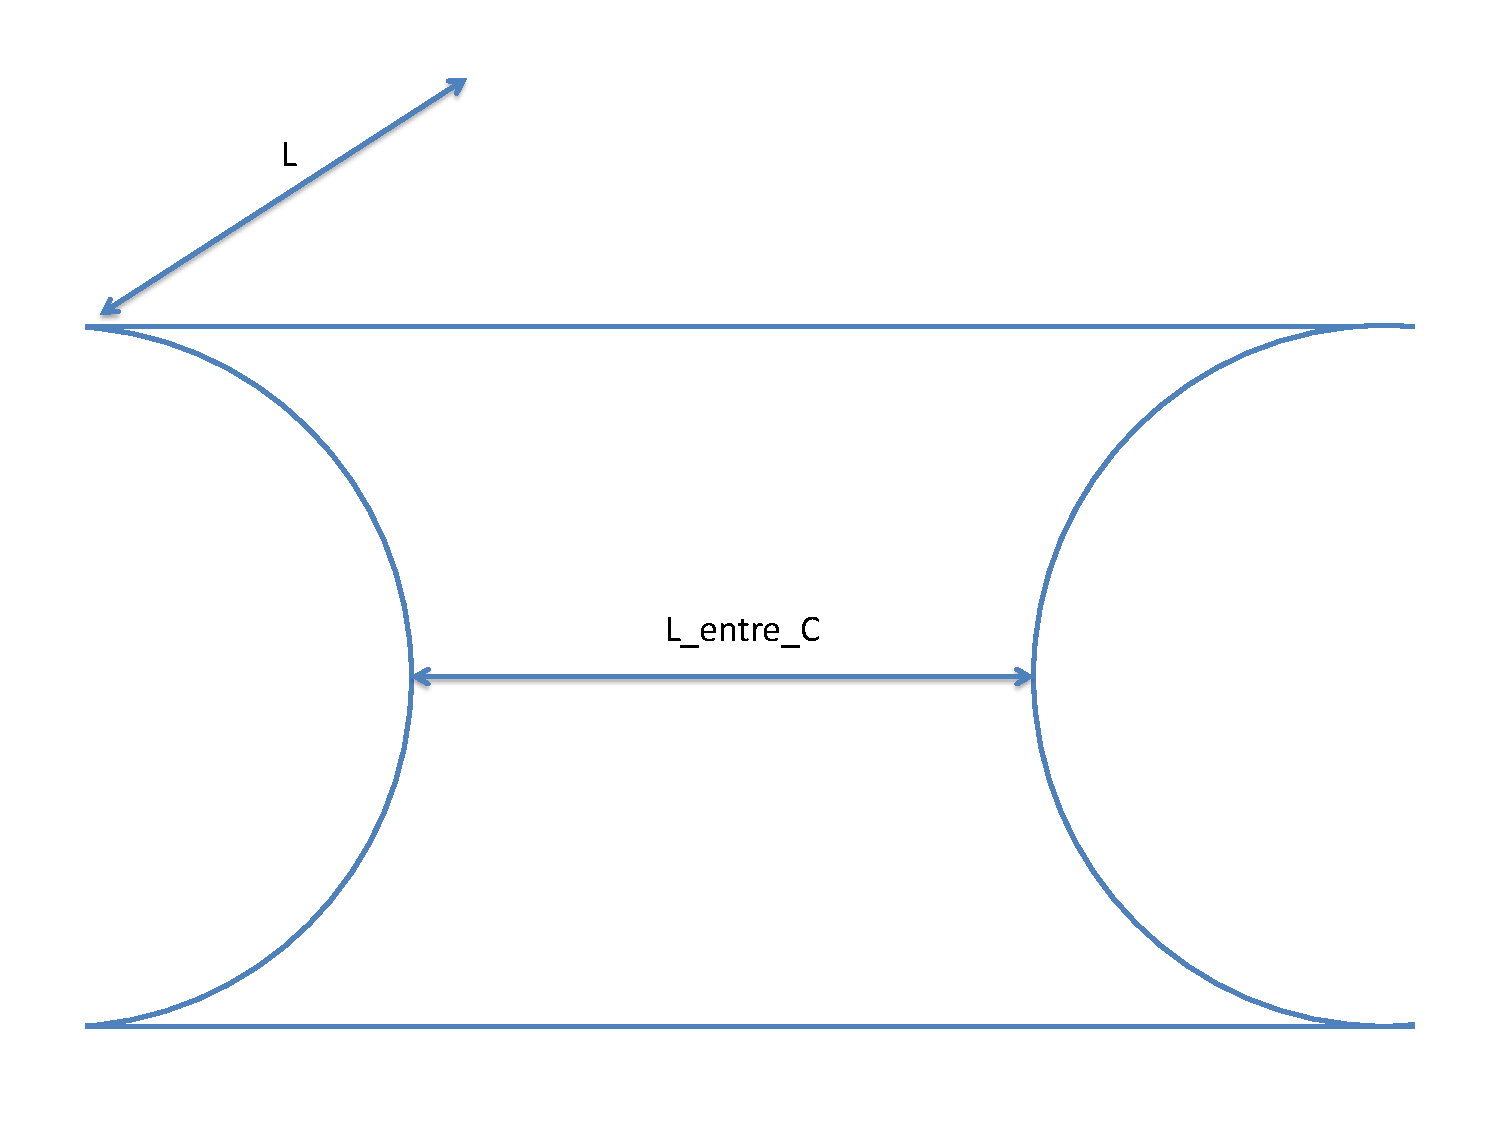
\includegraphics[scale=0.35]{PHOTO/Shema_conf_geo.pdf}
\label{conf_geo}
\end{figure}



\begin{figure}[!h]
\centering
\caption{Maillage}
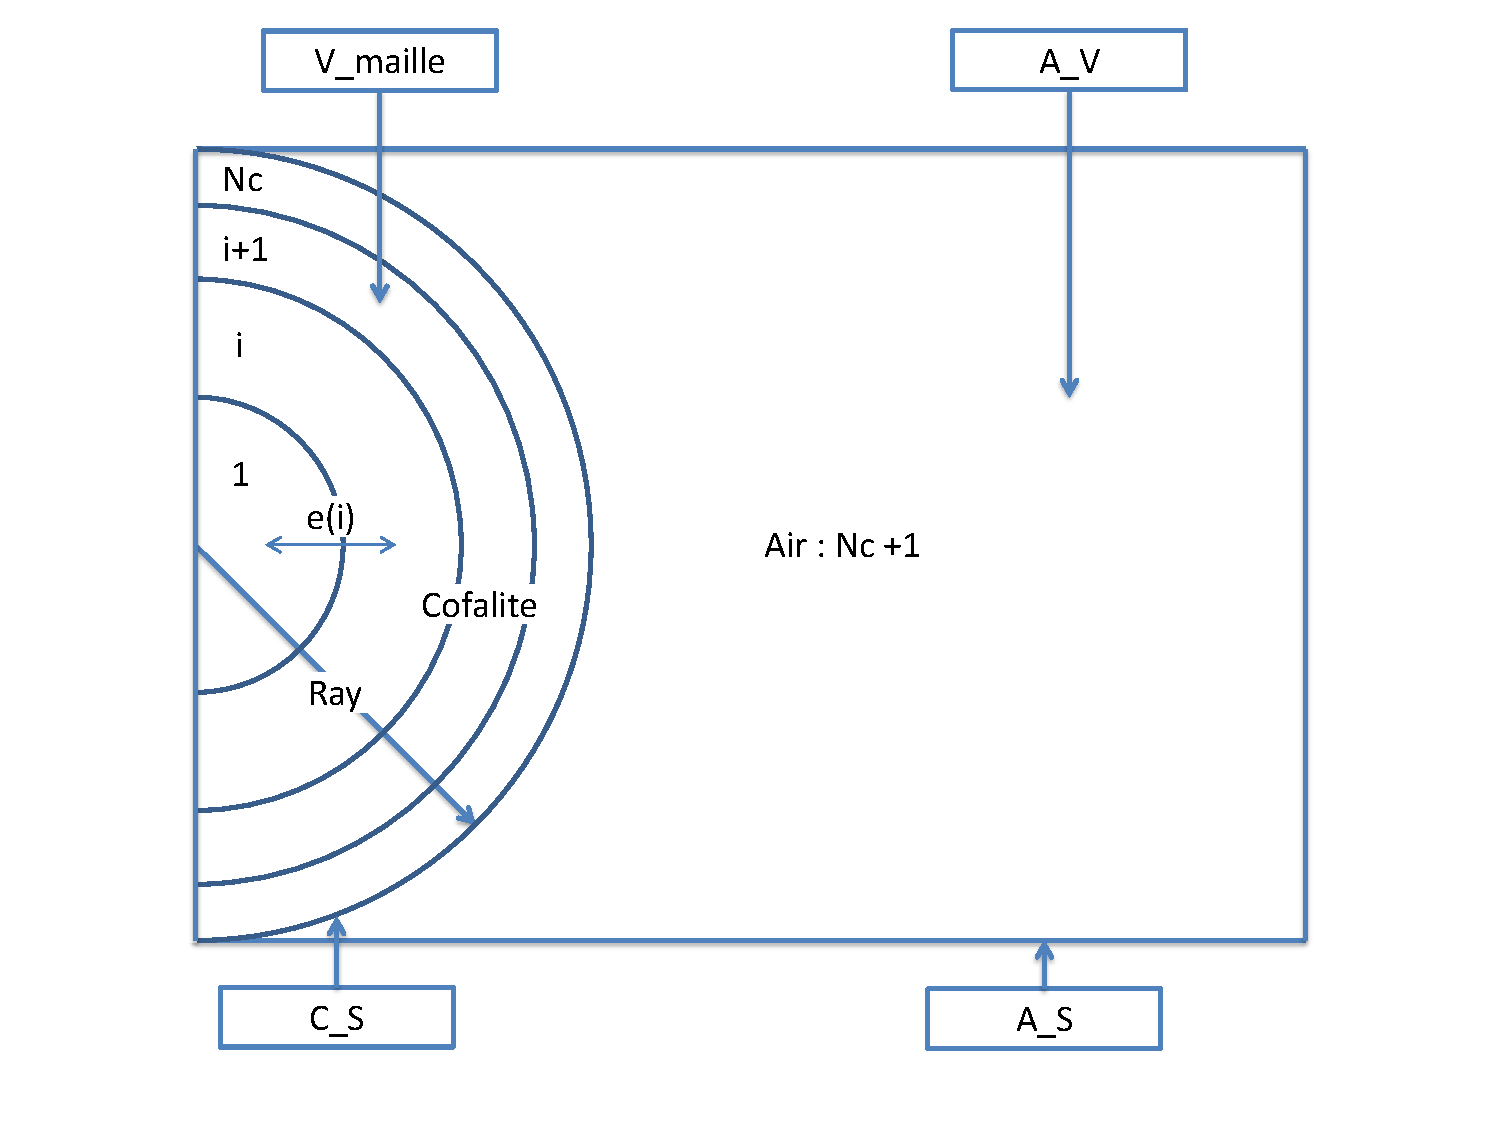
\includegraphics[scale=0.5]{PHOTO/Shema_maillage.pdf}
\label{maillage}
\end{figure}



\newpage


\section{Équations physiques résolues}
\textcolor{red}{LES ECRIRES}


\section{Variables d'entrées et de sorties}

	\subsection{Variables d'entrées}
	
		\subsubsection{Géométriques}
		
		Nous avons laissé, à l'utilisateur, une certaine marge de manœuvre pour adapter l'échangeur. 
		Ainsi, il peut fixer le rayon de chaque tubes de Cofalite. C'est la variable "Ray". 
		Il peut fixer la distance entre deux tubes sur le plan horizontale. C'est la variable "L\_entre\_C".
		
		Nous avons considéré que les contraintes d'espace sont plus déterminante au niveau de la surface au sol et moins sur le plan de la hauteur. De ce fait, l'utilisateur doit rentrer ses conditions sur la largeur et la profondeur de l'échangeur. Comme nous ne pouvons pas prédéterminer la hauteur de notre stockage il est fortement possible que celle-ci soit très importante. Par conséquent, ci celle ci ne lui convient pas, il devra soit augmenter la surface au sol, soit diminuer la température de consigne.\textcolor{red}{ Nous avons cependant rajouter une variable d'entrée intitulé "Hauteur\_max" qui permet de stopper de le code en cas de dépassement et donner un message d'erreur à l'utilisateur.}
		La variable de la profondeur s'intitule "L"; celle de la largeur "largeur".
		
		
		\subsubsection{Physique}
		
		Pour le stockage, nous devons mettre en place trois échangeurs (un entre chaque compresseur). De ce fait, L'air sort à une pression et température différente. 
		
		Nous avons fixer la pression pour trois valeurs différentes qui sont celle indiquer sur le schéma \ref{sh_fonc}, c'est à dire 4, 27 et 70 bar. L'utilisateur devra donc en indiquer une. Celle-ci permettra de considérer les propriétés de l'air à celle ci en fonction de la température.
		\textcolor{red}{ il faut faire le destockage à 50 bar!!!!!}\\
		
				
		Pour ce qui est de la température, l'on doit fixer la valeur de l'air. C'est la variable nommé "T\_entree". Nous avons fait un petit programme EES qui permet de les calculer. Il suffit de régler le rendement isentropique et \textcolor{red}{la température de sortie de l'air après passage dans les échangeurs.}
		Il faut également donner la température initiale de Cofalite (autour de 298K qui est la température de l'air à l'extérieur)
		
		\textcolor{red}{Pour le destockage, nous lirons la température du Cofalite après le stockage avec un éventuelle temps d'attente entre le stockage et destockage. En effet, la conductivité de celui ci est de $2 W.m^{-1}.K^{-1}$ et par conséquent, il existe un gradient de température au sein même du matériau.}\\
		
		Nous indiquerons aussi le débit d'entrée du Cofalite dans l'échangeur. Pour le stockage les données nous indique du $108kg.s^{-1}$, tendis que pour le destockage nous avons du $417kg.s^{-1}$ (voir tableau \ref{tab1}). 
		
		\subsubsection{Discrétisation}
			\paragraph{En espace :}
			
		L'utilisateur peut régler le nombre de maille sur le Cofalite avec la variable "Nc". Augmenter ce nombre rajoute de la précision sur le gradient de température au sein du matériau mais, de ce fait, améliore également la précision sur la température de sortie de l'air. Cependant, le temps de calcule augmente grandement. C'est pourquoi nous laissons l'utilisateur choisir en fonction de ses préférences. Attention, Nc doit avoir une valeur minimal de 3 pour que le code converge.
			\paragraph{En temps :}
		L'utilisateur fixe le temps de l'expérience, variable intitulé "T\_max". Pour le stockage nous avons un temps au alentour de $9\sim12$ heures (Heures creuses) et un temps de destockage de 3 heures (Heures pleines). 
		
		Nous indiquons le pas de temps. Le programme est assez robuste donc il peut être assez élevé, mais attention, cela reste du semi-implicite. \textcolor{red}{Une analyse de sensibilité sera faite plus loin}.
		
		
			  
\section{Organigramme}
	Nous présentons ici les organigrammes qui expliquent le fonctionnement de notre code.\\
	
	\textcolor{red}{ (à compléter/modifier)}
	Ci-dessous le fonctionnement de la principale subroutine "element" qui permet de résoudre le système pour chaque pas de temps.
	
\begin{figure}[!h]
	\centering
	\caption{Organigramme de la subroutine "element"}
	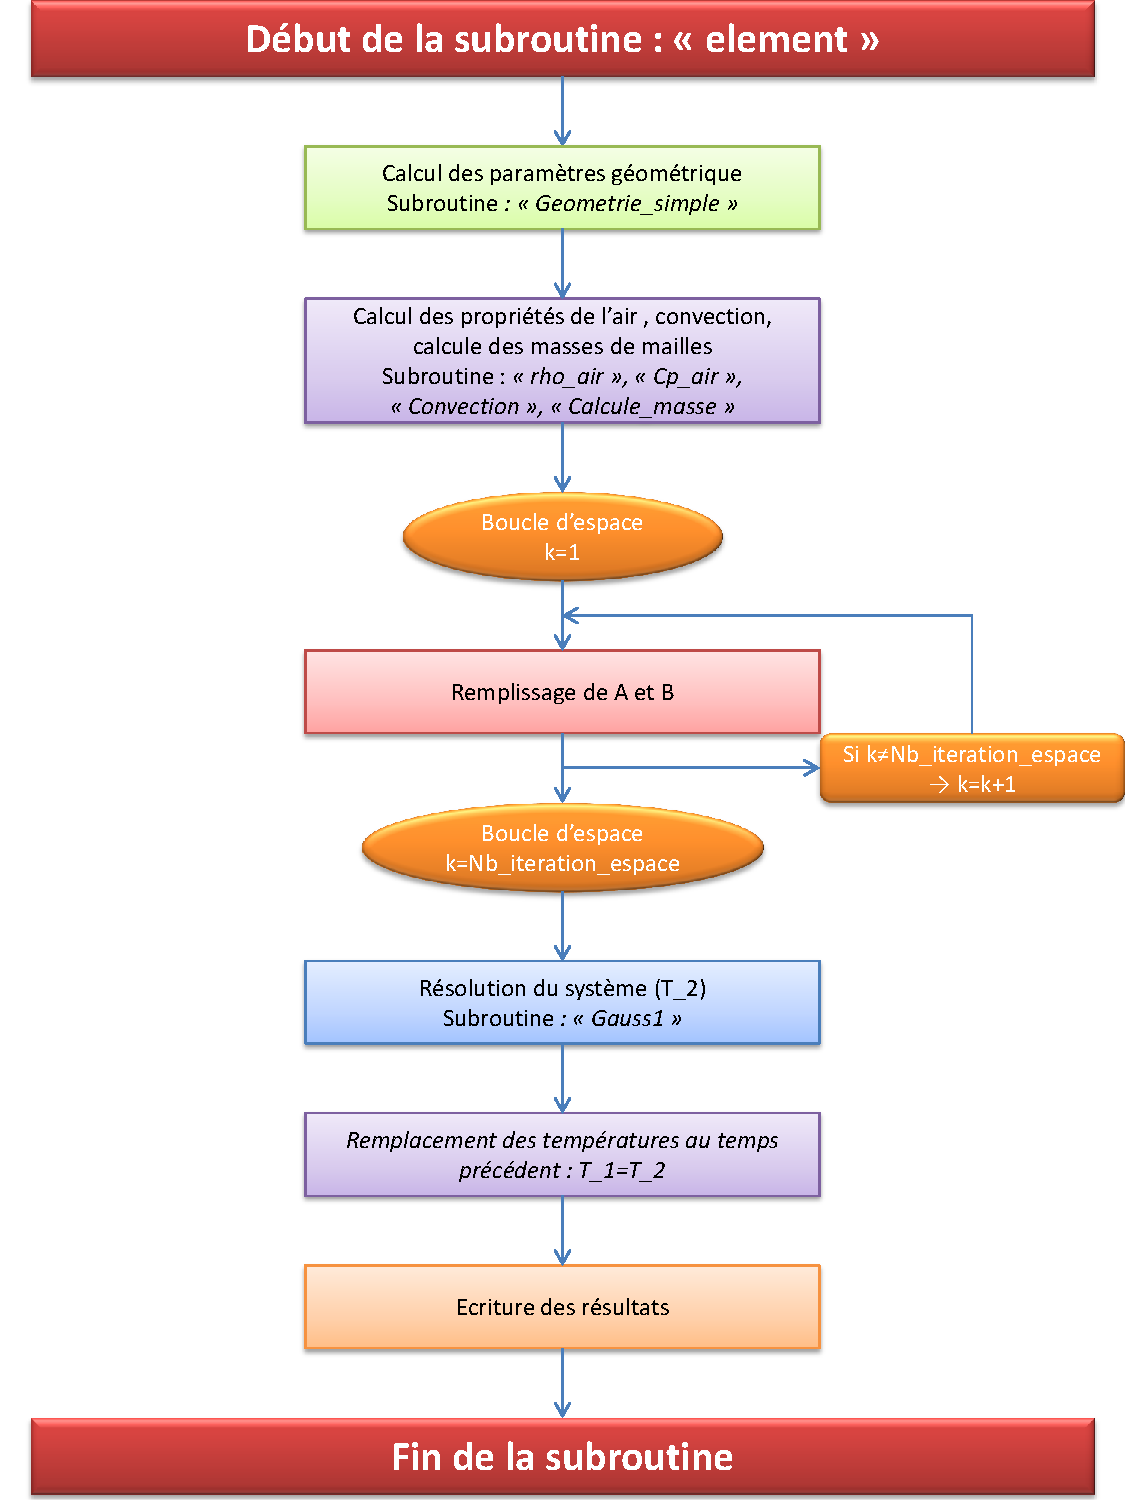
\includegraphics[scale=0.75]{PHOTO/Organigramme_element.pdf}
	\label{orgasme_element}
\end{figure}
	
		
	\newpage
	
	
		
		
\section{Vérification du code}		
		
Plusieurs simulations peuvent témoigner de la validité du code.

\subsection{Convergence}
		
Afin de tester la convergence des résultats, il convient de tester la convergence de la température du cofalit avec un temps de simulation suffisamment long.
Ainsi, le temps de simulation a été fixé à $1.10^{7}s$ avec un pas de temps de 10 secondes, pour une température d'air en entrée de 570K, et une température initiale de cofalit de 298K.
Le nombre de tube sur la hauteur a été fixé a 20 afin que le temps de simulation soit réduit au minimum.
Ainsi, les résultats affiché donne une température du cofalit a 570K quelque soit la maille considérée. La convergence du code est donc bien justifiée ici.

\subsection{Coherence du code}

Afin de vérifier la cohérence du code, la température de l'air en entrée a été fixé à la même valeur que celle du cofalit initialement.
Ainsi, quelque soit le temps de simulation, la température de l'air et du cofalit ne doit pas varier, et le transfert de chaleur doit être nul. 
Cependant, après simulation, la valeur du flux est de $8,7.10^{-6}J$, pour un temps de simulation de 100s, et avec 20 tubes de cofalit en hauteur.

